\subsection{Modelo MM1 en Python}

Para analizar el rendimiento del modelo, variamos la tasa de arribos ($T_a$) en base a la tasa de servicio ($T_s$), y
la capacidad de la cola ($cap$).

Realizaremos 100 simulaciones de 1000 clientes cada una y promediamos los siguientes estadísticos:
\begin{itemize}
    \item Promedio de clientes en el sistema ($q(n)+u(n)$)
    \item Cantidad de clientes en cola en promedio ($q(n)$)
    \item Demora promedio esperada en cola ($d(n)$)
    \item Tiempo promedio en el sistema ($d(n)+s(n)$)
    \item Ocupación del servidor ($u(n)*100\%$)
    \item Probabilidad de denegación del servicio. ($p(den)$)
    \item Probabilidad de encontrar n clientes en cola. ($p(Q(t)=n)\times100\%$)
\end{itemize}

\subsubsection[cap = 0]{$cap = 0$}

Los parámetros $d(n)$, $q(n)$ y $p(Q(t)=n)\times100\%$ no aplican cuando la capacidad de la cola es 0.
El promedio de clientes en sistema es en este caso, equivalente al factor de uso del servicio.

\begin{tabular}{||c||c|c|c||}
    \hline \hline
    $\frac{T_a}{T_s}\times100\%$ [\%] & $d(n)+s(n)$ [min] & $u(n)\times100\%$ [\%] & $p(den)$ [\%] \\
    \hline \hline
    25 & $$ & $$ & $$ \\
    \hline
    50 & $$ & $$ & $$ \\
    \hline
    75 & $$ & $$ & $$ \\
    \hline
    100 & $$ & $$ & $$ \\
    \hline
    125 & $$ & $$ & $$ \\
    \hline \hline
\end{tabular}

\subsubsection[cap = 2]{$cap = 2$}

\begin{tabular}{||c||c|c|c|c|c|c||}
    \hline \hline
    $\frac{T_a}{T_s}\times100\%$ [\%] & $q(n)+u(n)$ [min] & $q(n)$ [clientes] & $d(n)$ [min] & $d(n)+s(n)$ [min] & $u(n)\times100\%$ [\%] & $p(den)$ [\%] \\
    \hline \hline
    25 & $$ & $$ & $$ & $$ & $$ & $$ \\
    \hline
    50 & $$ & $$ & $$ & $$ & $$ & $$ \\
    \hline
    75 & $$ & $$ & $$ & $$ & $$ & $$ \\
    \hline
    100 & $$ & $$ & $$ & $$ & $$ & $$ \\
    \hline
    125 & $$ & $$ & $$ & $$ & $$ & $$ \\
    \hline \hline
\end{tabular}

\begin{figure}[H]
  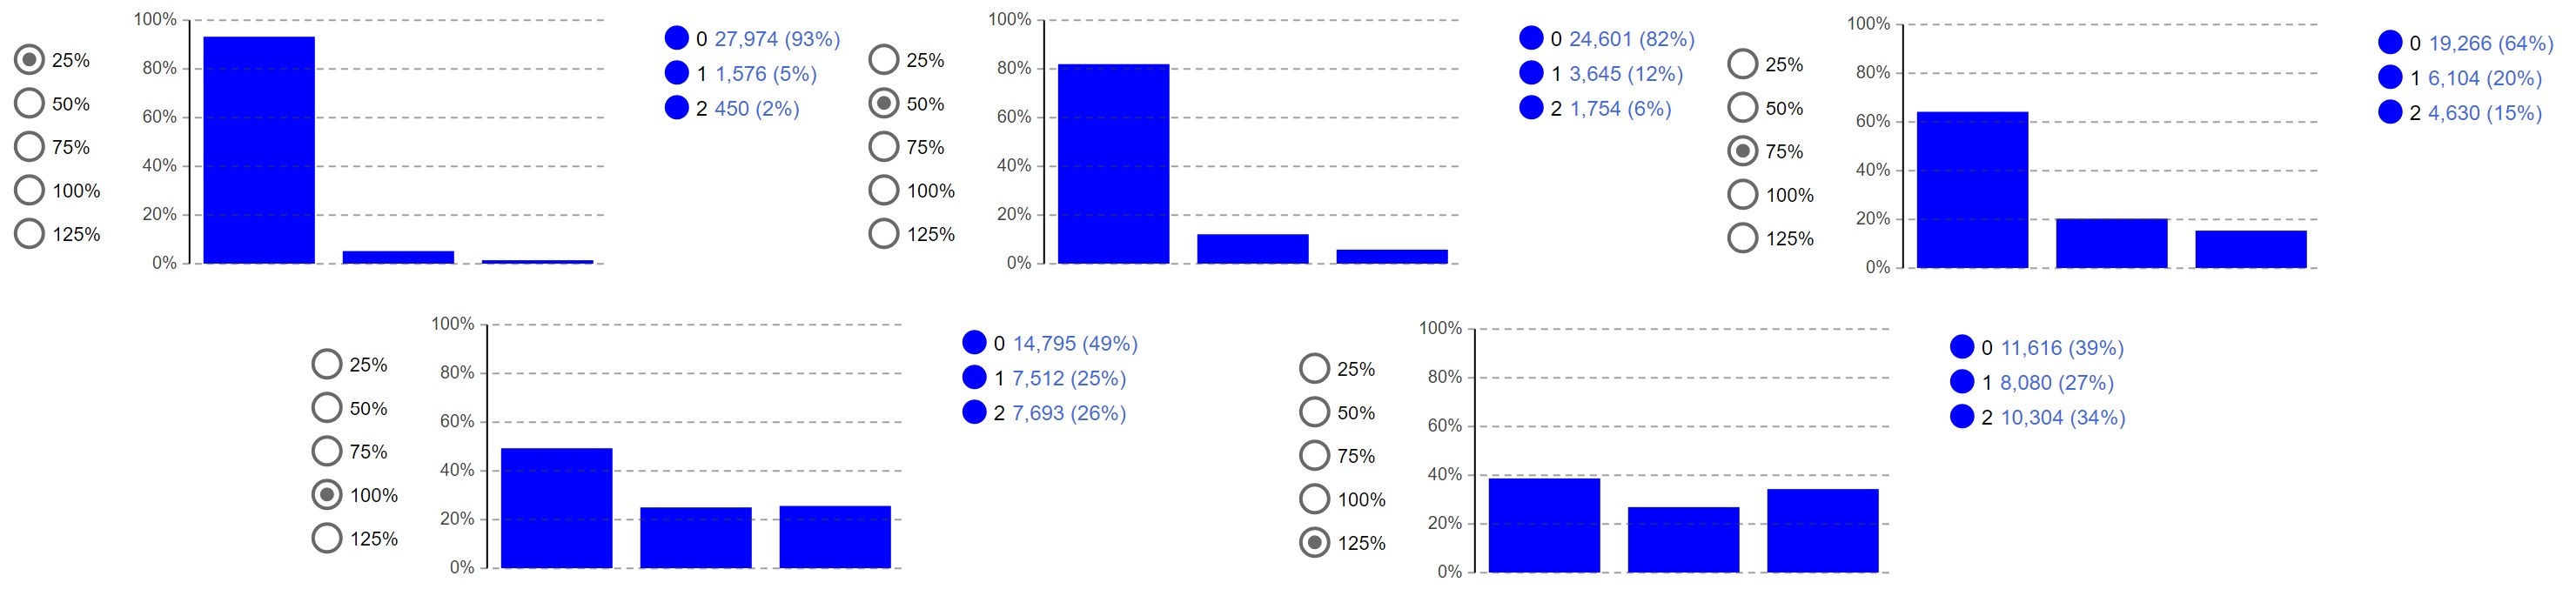
\includegraphics[width=\linewidth]{images/anylogic-colas-2}
  \caption{Probabilidad de encontrar n clientes en cola.}
\end{figure}

\subsubsection[cap = 5]{$cap = 5$}

\begin{tabular}{||c||c|c|c|c|c|c||}
    \hline \hline
    $\frac{T_a}{T_s}\times100\%$ [\%] & $q(n)+u(n)$ [min] & $q(n)$ [clientes] & $d(n)$ [min] & $d(n)+s(n) [min]$ & $u(n)\times100\%$ [\%] & $p(den)$ [\%] \\
    \hline \hline
    25 & $$ & $$ & $$ & $$ & $$ & $$ \\
    \hline
    50 & $$ & $$ & $$ & $$ & $$ & $$ \\
    \hline
    75 & $$ & $$ & $$ & $$ & $$ & $$ \\
    \hline
    100 & $$ & $$ & $$ & $$ & $$ & $$ \\
    \hline
    125 & $$ & $$ & $$ & $$ & $$ & $$ \\
    \hline \hline
\end{tabular}

\begin{figure}[H]
  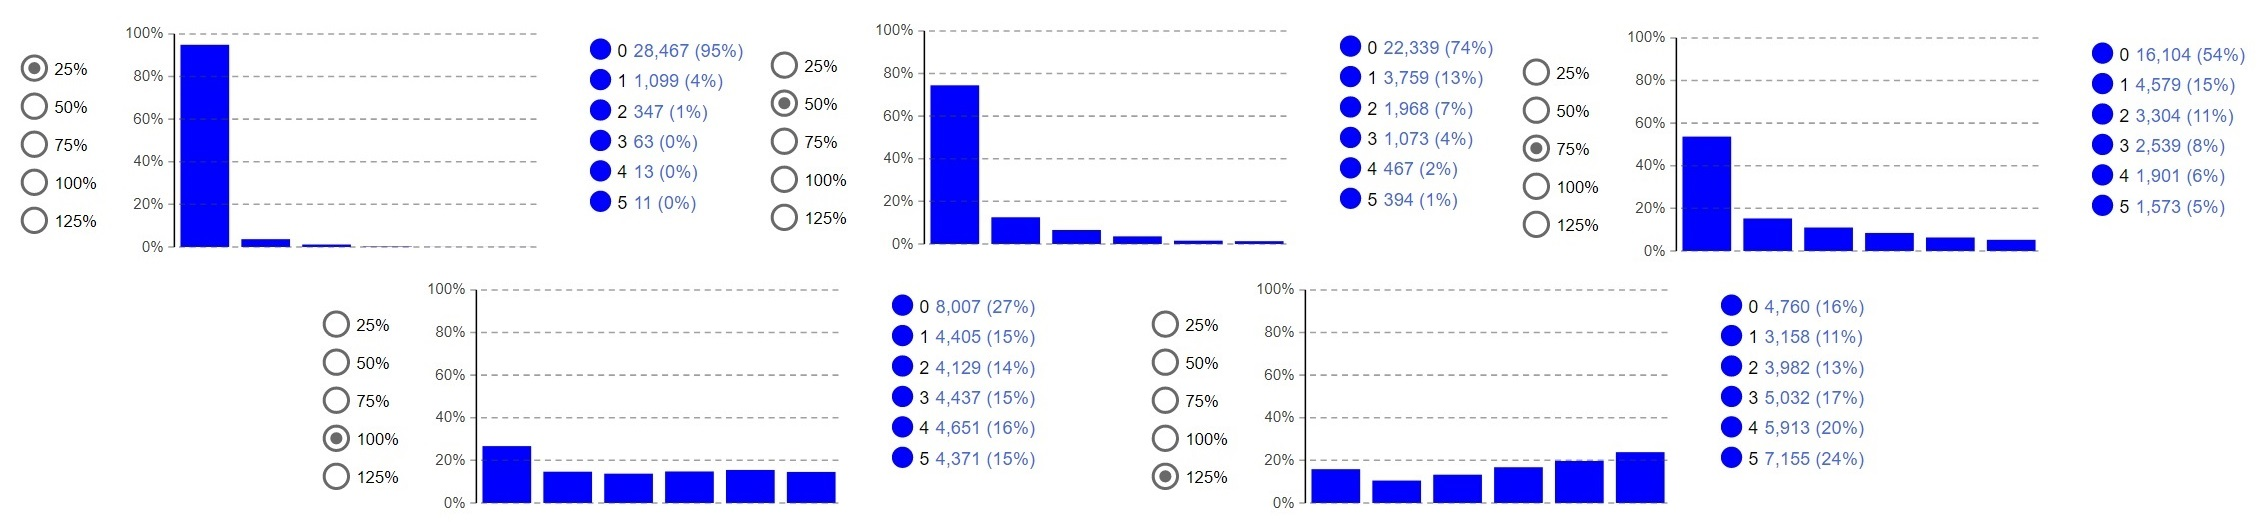
\includegraphics[width=\linewidth]{images/anylogic-colas-5}
  \caption{Probabilidad de encontrar n clientes en cola.}
\end{figure}

\subsubsection[cap = 10]{$cap = 10$}

\begin{tabular}{||c||c|c|c|c|c|c||}
    \hline \hline
    $\frac{T_a}{T_s}\times100\%$ [\%] & $q(n)+u(n)$ [min] & $q(n)$ [clientes] & $d(n)$ [min] & $d(n)+s(n) [min]$ & $u(n)\times100\%$ [\%] & $p(den)$ [\%] \\
    \hline \hline
    25 & $$ & $$ & $$ & $$ & $$ & $$ \\
    \hline
    50 & $$ & $$ & $$ & $$ & $$ & $$ \\
    \hline
    75 & $$ & $$ & $$ & $$ & $$ & $$ \\
    \hline
    100 & $$ & $$ & $$ & $$ & $$ & $$ \\
    \hline
    125 & $$ & $$ & $$ & $$ & $$ & $$ \\
    \hline \hline
\end{tabular}

\begin{figure}[H]
  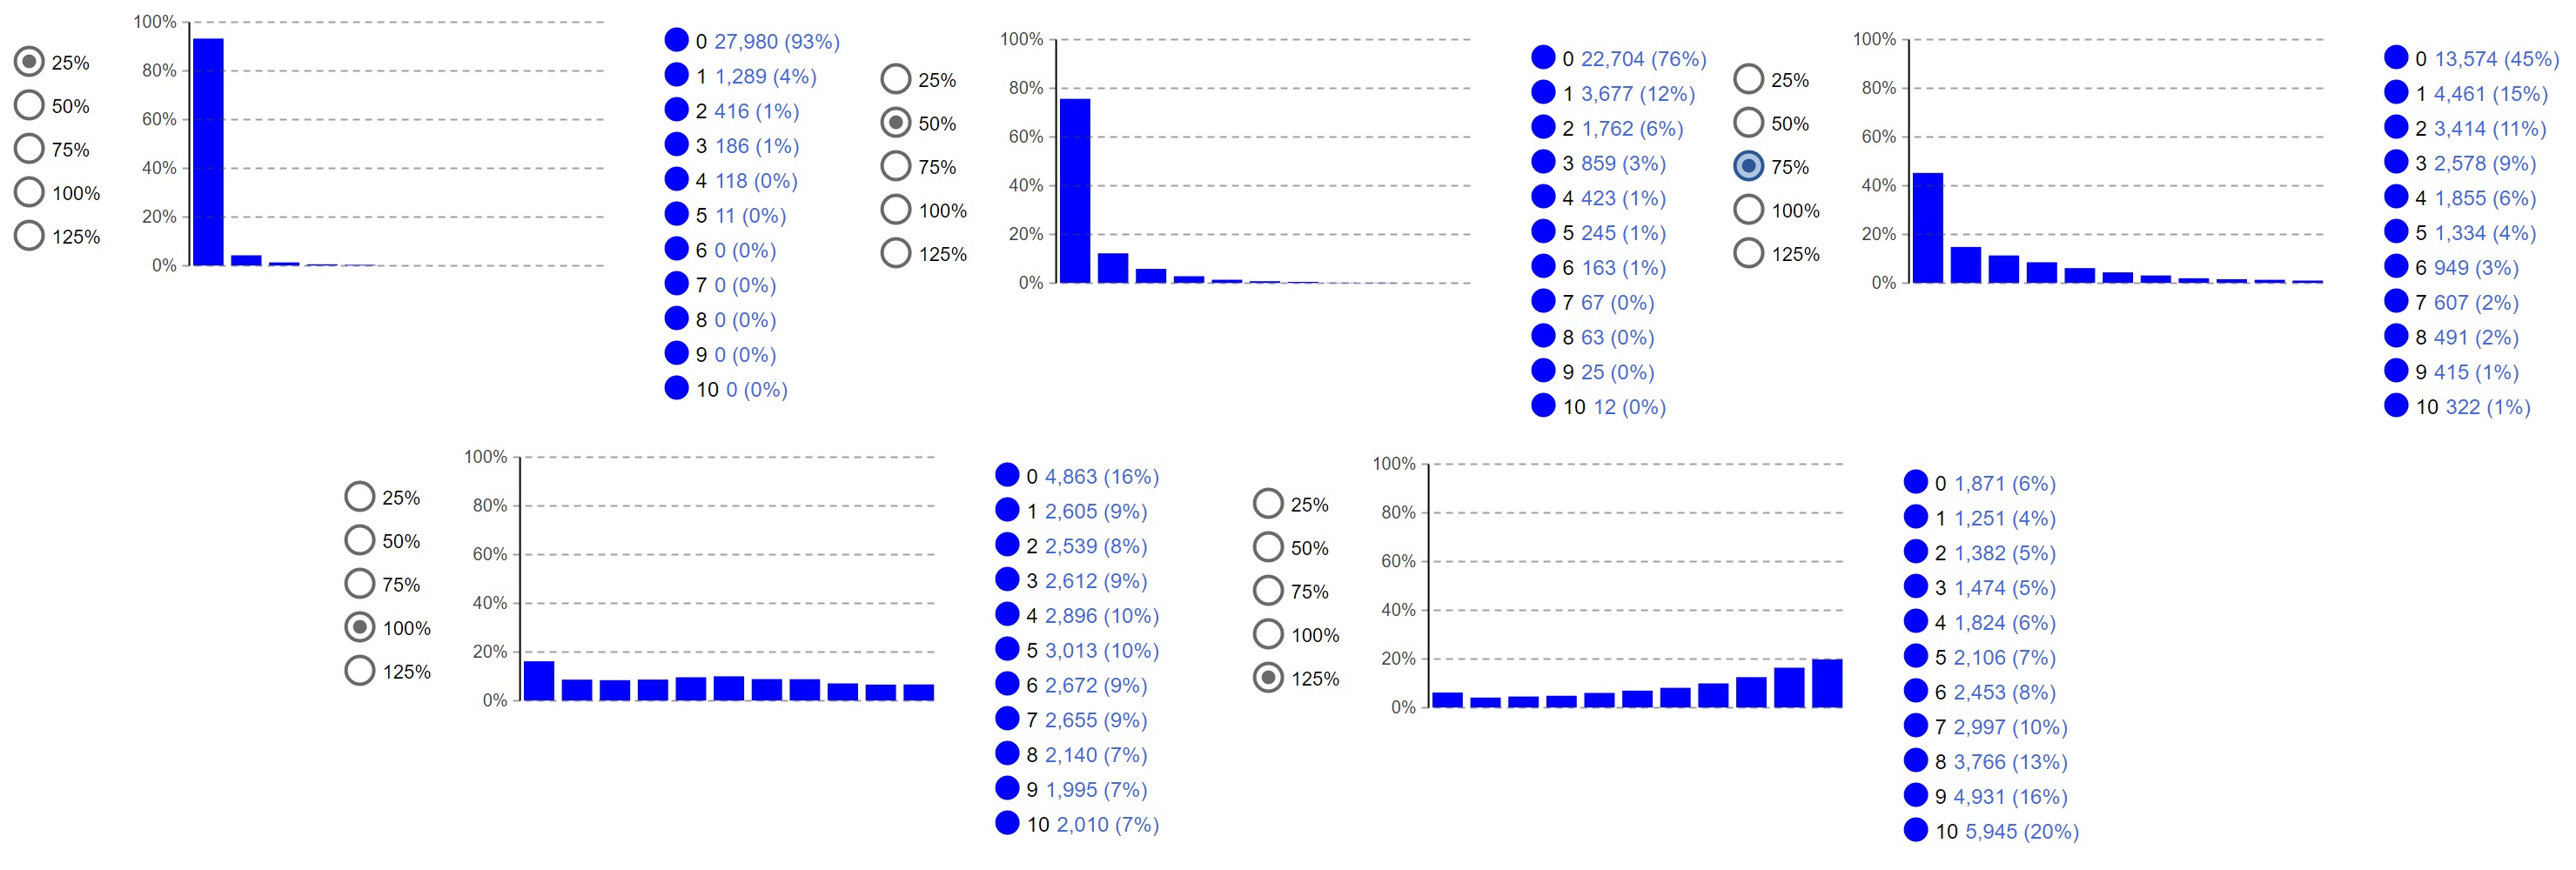
\includegraphics[width=\linewidth]{images/anylogic-colas-10}
  \caption{Probabilidad de encontrar n clientes en cola.}
\end{figure}

\subsubsection[cap = 50]{$cap = 50$}

\begin{tabular}{||c||c|c|c|c|c|c||}
    \hline \hline
    $\frac{T_a}{T_s}\times100\%$ [\%] & $q(n)+u(n)$ [min] & $q(n)$ [clientes] & $d(n)$ [min] & $d(n)+s(n) [min]$ & $u(n)\times100\%$ [\%] & $p(den)$ [\%] \\
    \hline \hline
    25 & $$ & $$ & $$ & $$ & $$ & $$ \\
    \hline
    50 & $$ & $$ & $$ & $$ & $$ & $$ \\
    \hline
    75 & $$ & $$ & $$ & $$ & $$ & $$ \\
    \hline
    100 & $$ & $$ & $$ & $$ & $$ & $$ \\
    \hline
    125 & $$ & $$ & $$ & $$ & $$ & $$ \\
    \hline \hline
\end{tabular}

\begin{figure}[H]
  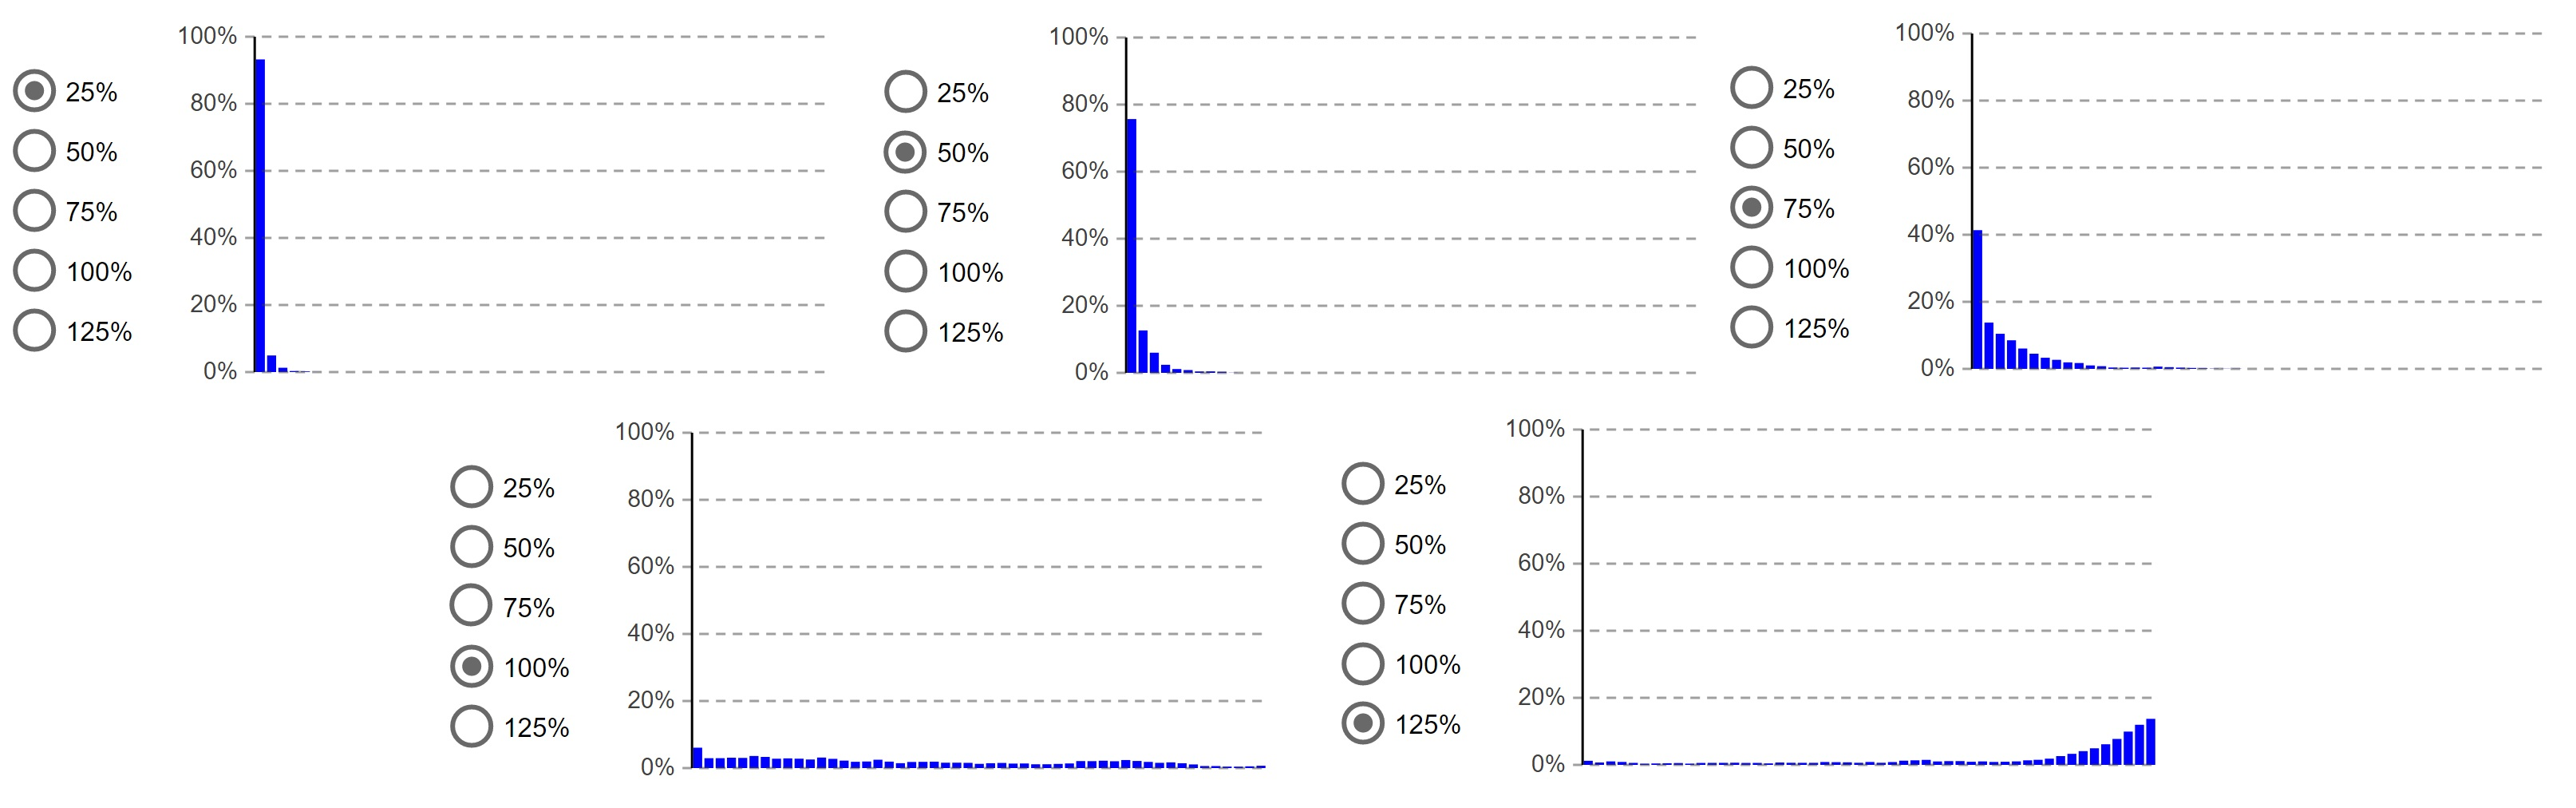
\includegraphics[width=\linewidth]{images/anylogic-colas-50}
  \caption{Probabilidad de encontrar n clientes en cola.}
\end{figure}

\subsubsection[cap = ∞]{$cap = \infty$}

En este caso no tenemos tope de clientes en la cola, entonces no hay probabilidad de denegación.

\begin{itemize}
    \item Promedio de clientes en el sistema ($q(n)+u(n)$)
    \item Cantidad de clientes en cola en promedio ($q(n)$)
    \item Demora promedio esperada en cola ($d(n)$)
    \item Tiempo promedio en el sistema ($d(n)+s(n)$)
    \item Ocupación del servidor ($u(n)*100\%$)
\end{itemize}

\begin{tabular}{||c||c|c|c|c|c|c||}
    \hline \hline
    $\frac{T_a}{T_s}\times100\%$ [\%] & $q(n)+u(n)$ [min] & $q(n)$ [clientes] & $d(n)$ [min] & $d(n)+s(n) [min]$ & $u(n)\times100\%$ [\%]\\
    \hline \hline
    25 & $0,331$ & $0,082$ & $0,653$ & $2,637$ & $24,866$ \\
    \hline
    50 & $0,995$ & $0,496$ & $1,978$ & $3,981$ & $49,949$ \\
    \hline
    75 & $2,924$ & $2,176$ & $5,778$ & $7,778$ & $74,845$ \\
    \hline
    100 & $23,853$ & $22,892$ & $45,548$ & $47,546$ & $96,121$ \\
    \hline
    125 & $127,97$ & $126,975$ & $203,476$ & $205,469$ & $99,563$ \\
    \hline \hline
\end{tabular}

\begin{figure}[H]
  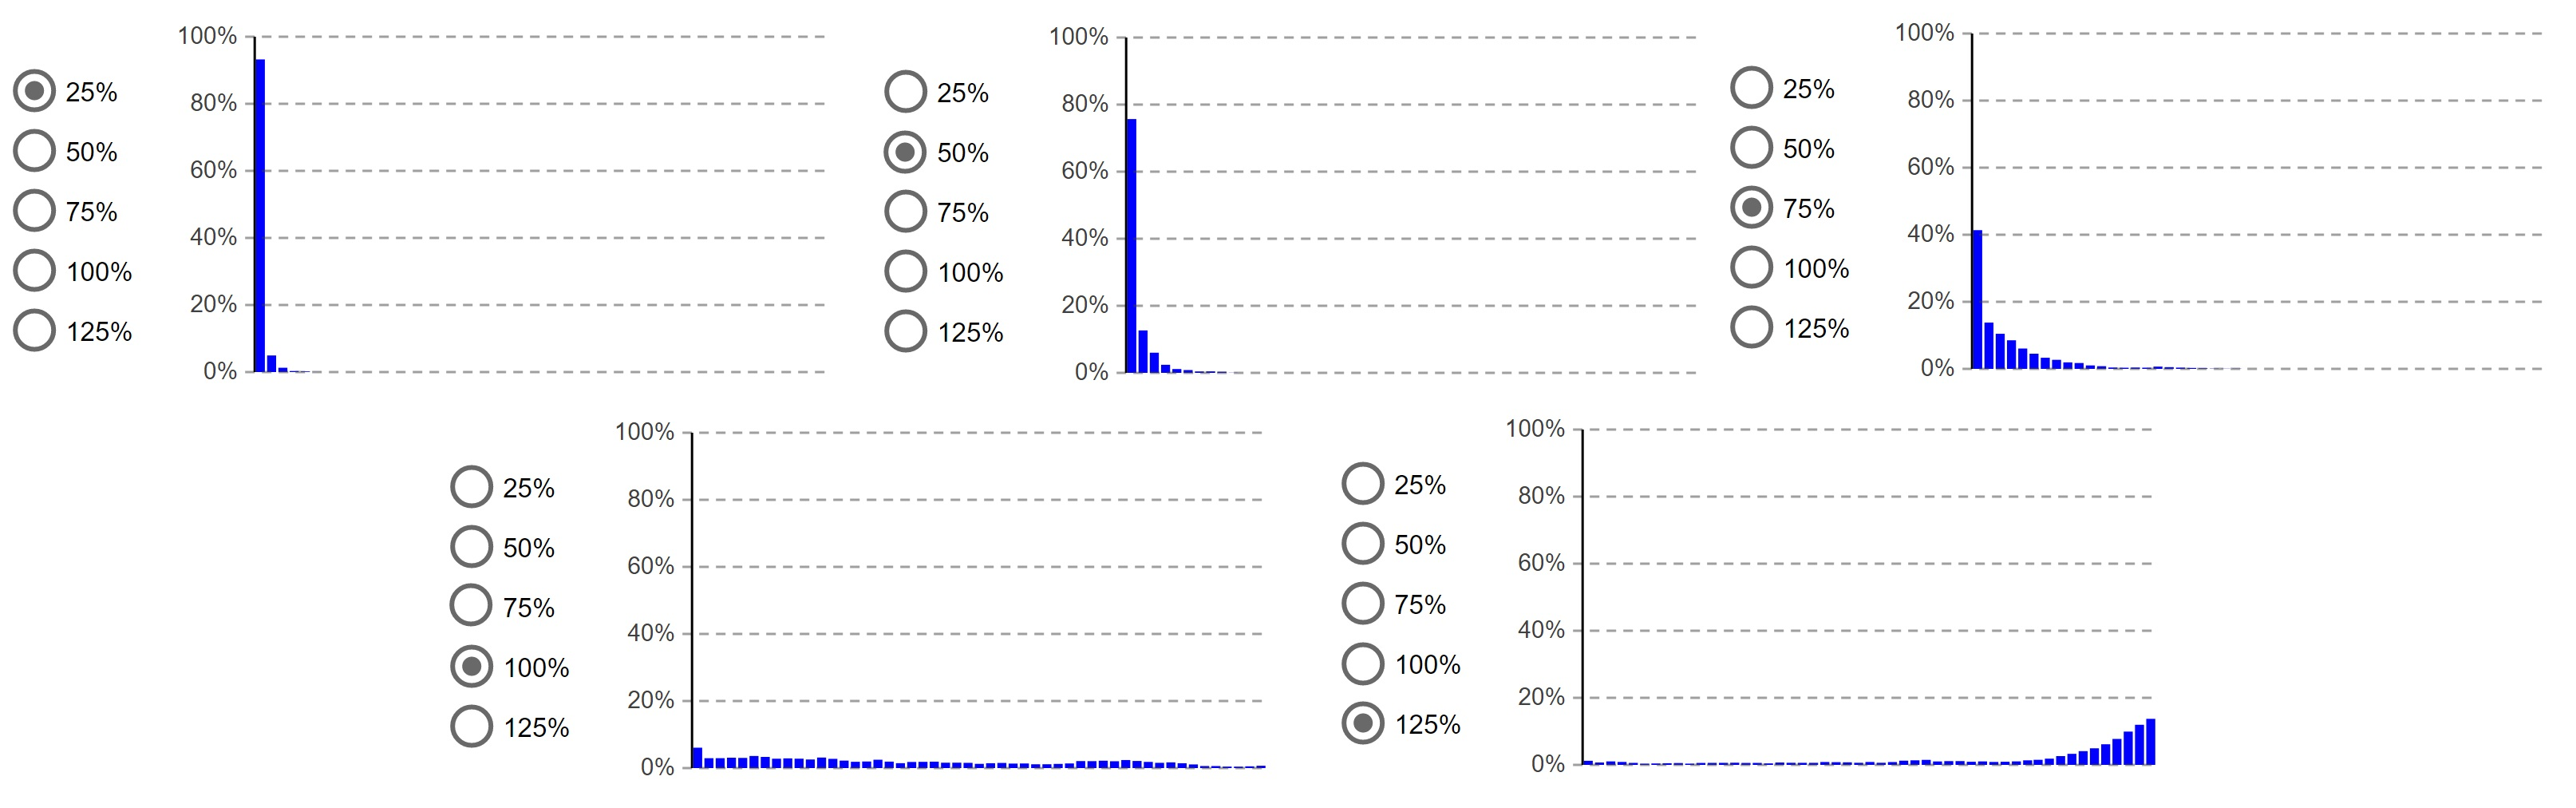
\includegraphics[width=\linewidth]{images/anylogic-colas-50}
  \caption{Probabilidad de encontrar n clientes en cola.}
\end{figure}

